\documentclass{beamer}
\usetheme{metropolis}           % Use metropolis theme

\usepackage{mathtools}
\usepackage{amsmath}

\useoutertheme{metropolis}
\useinnertheme{metropolis}
\usefonttheme{metropolis}
\usecolortheme{beaver} 

\usefonttheme{professionalfonts} % required for mathspec
\usepackage{mathspec}
% set math to default LaTeX font
\setsansfont[BoldFont={Fira Sans},
Numbers={OldStyle}]{Fira Sans Light}

\title{Shape Synthesis from Sketches via Procedural Models and Convolutional Networks}
\date{}
\author{Haibin Huang, Evangelos Kalogerakis, Ersin Yumer, Radomir Mech}
\institute{Presentation by Julien}
\begin{document}
    \maketitle
    
    \section{Procedural Modeling}
    
    \begin{frame}{Procedural Modeling}
        Synthesize 2D or 3D models with a set of parameters.
        \begin{figure}
            \centering
            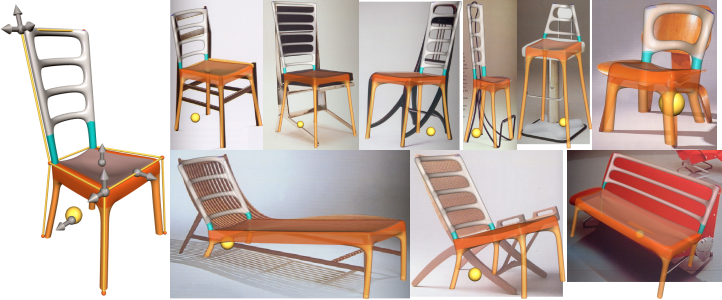
\includegraphics[width=0.9\textwidth]{images/GML-Stuhl-Template.png}
            \caption{Procedurally Modeled Chairs {\tiny (from Sven Havemann, Wikipedia)}}
            \label{fig:PM_Chair}
        \end{figure}
    \end{frame}
  
    \begin{frame}[standout]
        \Large
        Idea: Learn to translate human sketches to Procedural Modeling parameters.
    \end{frame}
    
    \begin{frame}{Human Sketches}
        A challenge of this approach is dealing with dramatic abstractions, simplifications, and exaggerations humans make when drawing objects.
        \begin{figure}
            \centering
            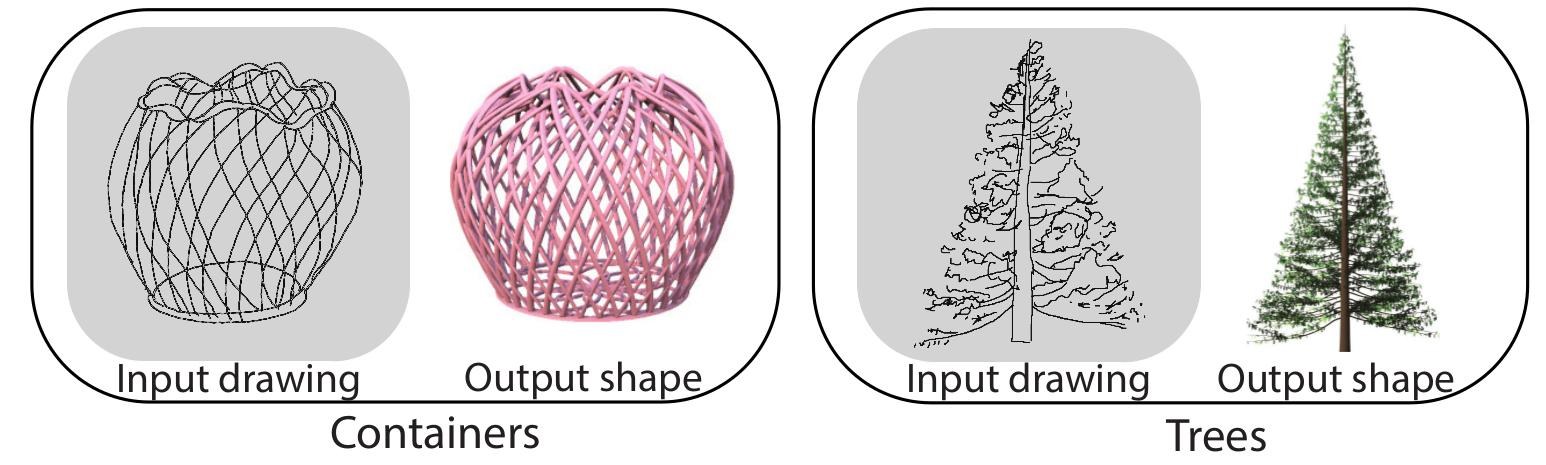
\includegraphics[width=\textwidth]{images/sketches.jpg}
            % \caption{Human Sketches}
            \label{fig:sketches}
        \end{figure}
        % Solution: use machine learning.
    \end{frame}
    
    \section{A Convolutional Neural Network Architecture}
    
    \begin{frame}{The Data}
        With a user study and careful curation of generated sketches, a synthetic dataset can be created for a model.
        \begin{figure}
            \centering
            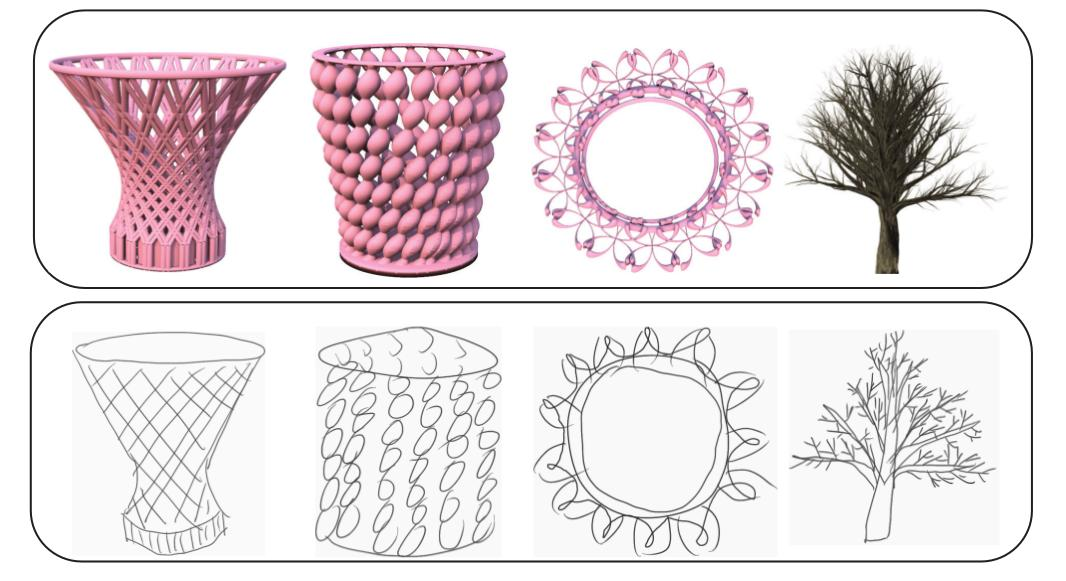
\includegraphics[width=0.9\textwidth]{images/user-sketch.jpg}
            % \caption{User Sketches}
            \label{fig:user-sketch}
        \end{figure}
    \end{frame}
    
    \begin{frame}{CNN Architecture}
        Composed of two distinct AlexNet CNN architectures.
        \begin{figure}
            \centering
            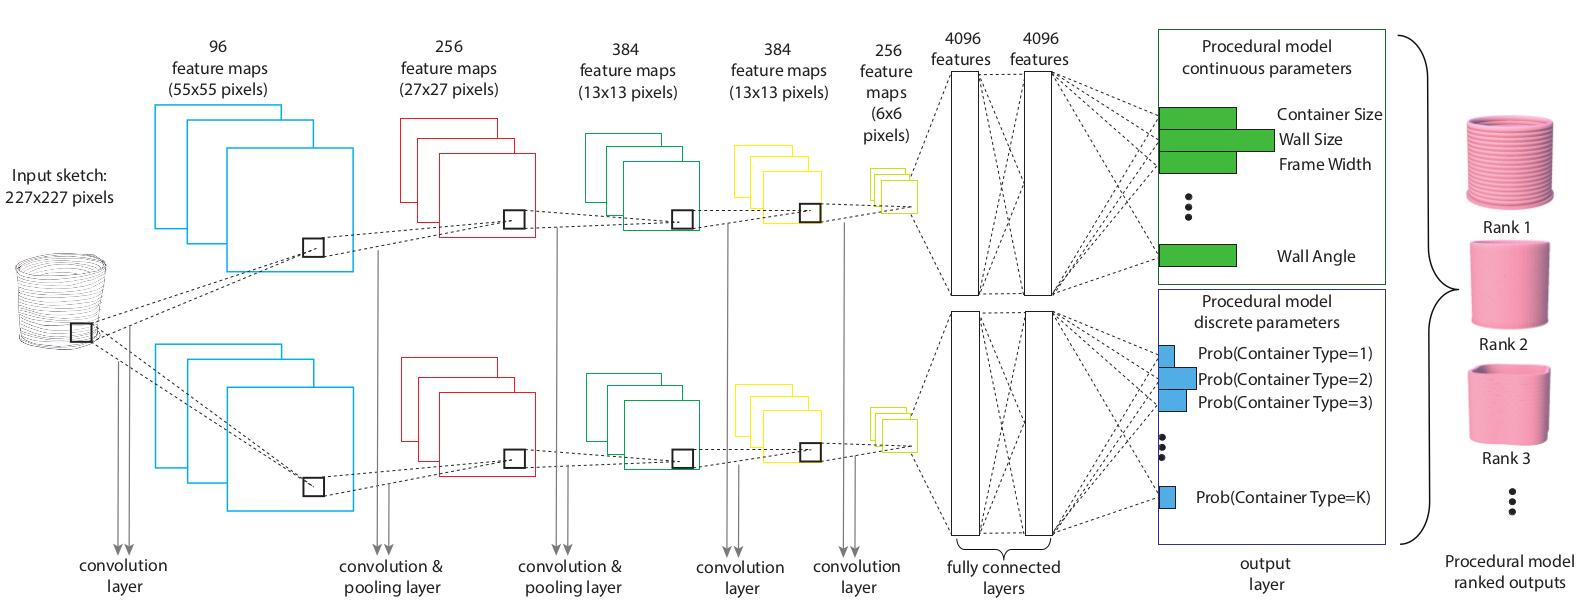
\includegraphics[width=\textwidth]{images/architecture.jpg}
            % \caption{CNN}
            \label{fig:architecture}
        \end{figure}
        One with additional layer for regression of continuous parameters, the other with additional layer for classification of discrete parameters.
    \end{frame}
    
    \begin{frame}{Pre-training}
        AlexNet pre-trained on ImageNet gives significant performance increase for free. 
        
        Image classification is a similar task, similar visual features will be useful for sketch $\to$ shape parameter task.
        
        The network can then be fine tuned by training end to end.
        
    \end{frame}
    
    \begin{frame}{Regression and Classification Layers}
        The regression layer estimates a normalized parameter $c$ within the range $[0,1]$ using a sigmoid.
        $$
        O_c = \frac{1}{1+\exp(-\mathbf{w}_c \cdot \mathbf{h}_L -b_c)}
        $$
        
        The classification layer estimates probabilities of each value of a discrete parameter $D_r$ using a softmax.
        $$
        P(D_r = d) =
        \frac{\exp(\mathbf{w}_{d,r} \cdot \mathbf{h}_L + b_{d,r})}
        {\exp(\sum_{d'}\mathbf{w}_{d',r} \cdot \mathbf{h}_L + b_{d',r})}
        $$
    \end{frame}
    
    
    \begin{frame}{Loss Functions}
    Loss function for $C$ continuous parameters over $S$ sketches in training data. Uses $L^2$ loss with $L^2$ regularization.
    $$
    E_\text{reg}(\mathbf{\theta}_1) = 
    \sum_{s=1}^{S} \sum_{c=1}^{C} \mathbf{1}_{\delta_{c,s}} 
    || O_{c,s}(\mathbf{\theta}_1) - \hat O_{c,s} ||^2
    + \lambda_1 || \mathbf{\theta}_1 ||^2
    $$
    
    Loss function for $R$ discrete parameters over $S$ sketches in training data. Uses logistic loss with $L^2$ regularization.
    $$
    E_\text{class}(\mathbf{\theta}_2) = 
    \sum_{s=1}^{S} \sum_{r=1}^{R} \log(P(D_{s,r} = \hat d_{s,r} \mid \mathbf{\theta}_2))
    + \lambda_2 || \mathbf{\theta}_2 ||^2
    $$
        
    \end{frame}
    
    \section{Results}
    
    \begin{frame}{At Runtime}
        GPU execution can predict PM parameters given a sketch in 1 to 2 seconds. 
        
        This is fast enough for near-interactive use.
        
        \begin{figure}
            \centering
            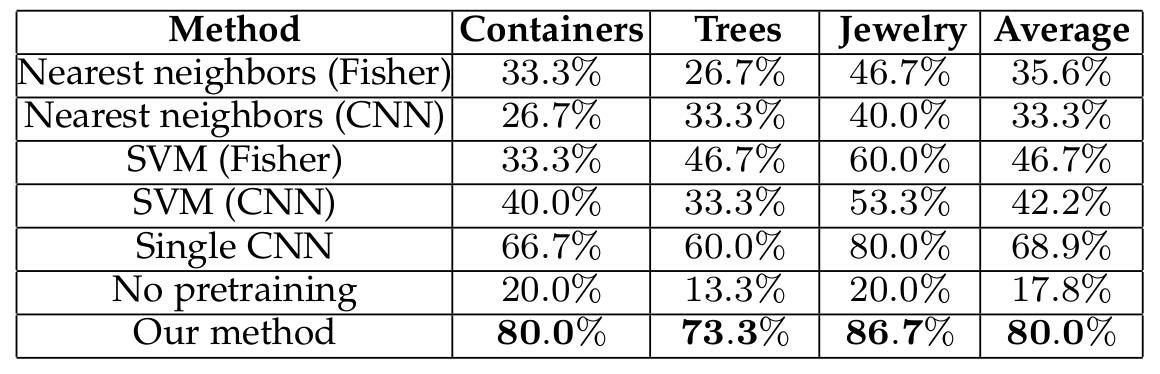
\includegraphics[width=0.8\textwidth]{images/table.jpg}
            \caption{Top-3 classification accuracy for discrete parameters}
            \label{fig:table}
        \end{figure}
    \end{frame}

    \begin{frame}{Results}
        \begin{figure}
            \centering
            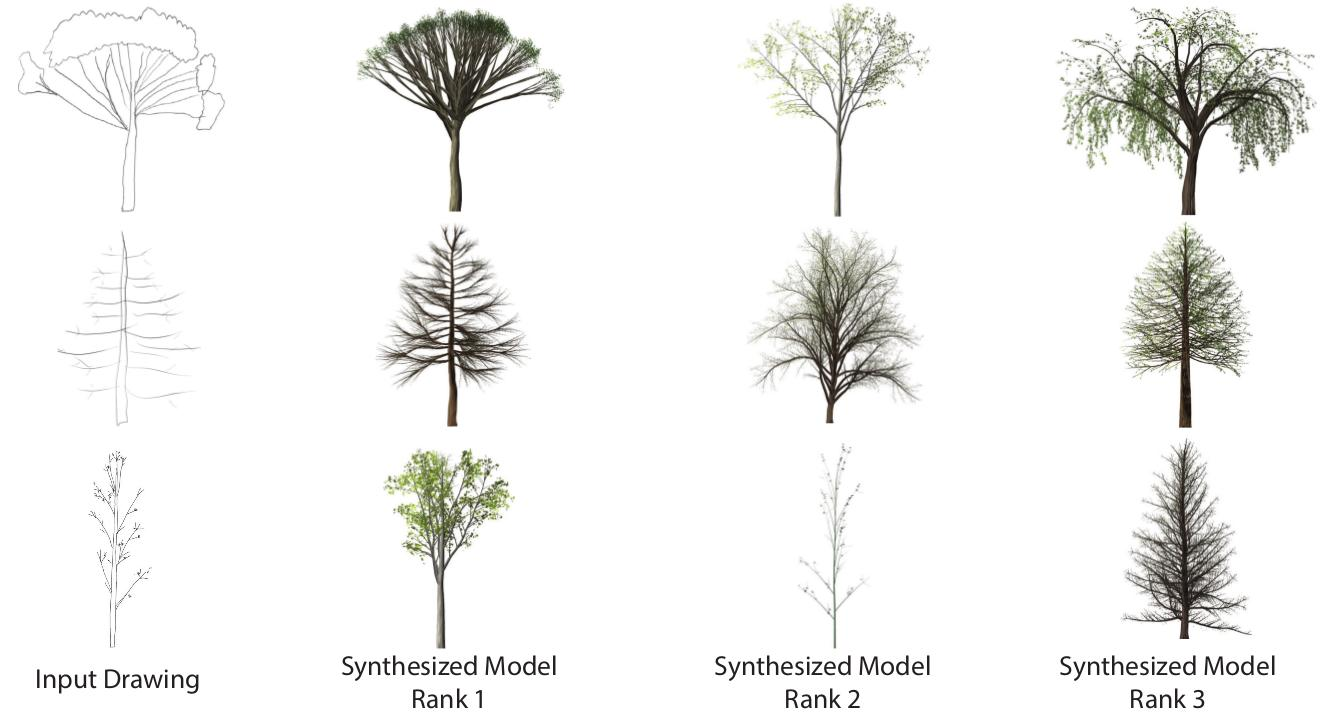
\includegraphics[width=\textwidth]{images/trees.jpg}
            % \caption{Trees}
            \label{fig:trees}
        \end{figure}
    \end{frame}
    
    \begin{frame}{Results}
        \begin{figure}
            \centering
            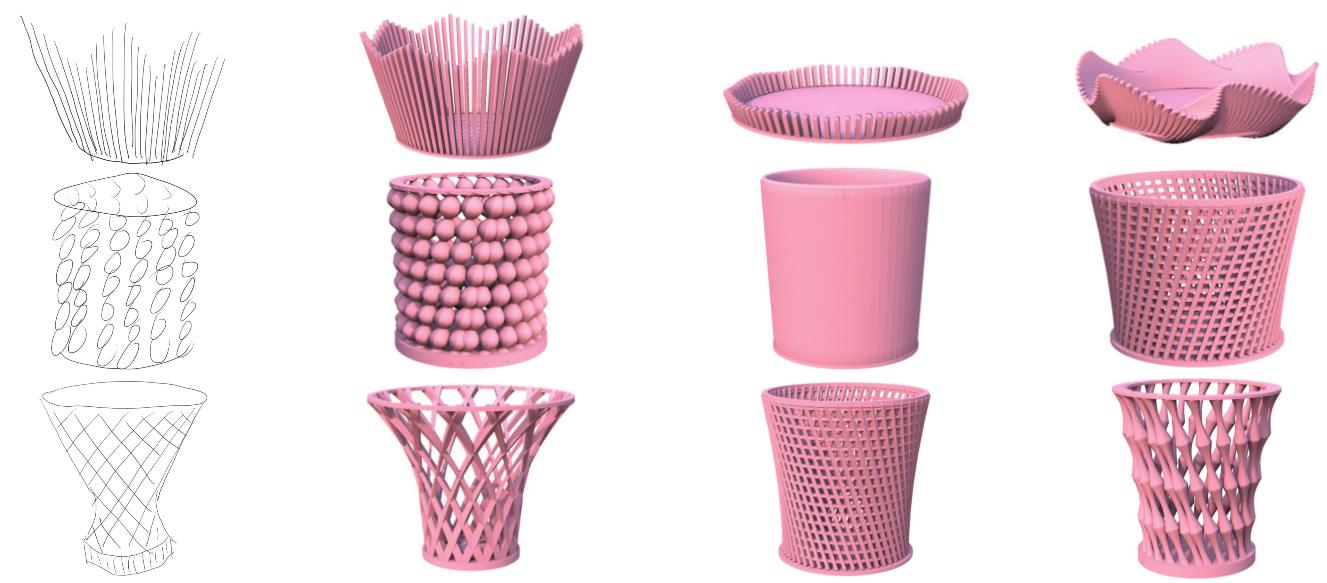
\includegraphics[width=\textwidth]{images/containers.jpg}
            % \caption{Containers}
            \label{fig:containers}
        \end{figure}
    \end{frame}
  
\end{document}